
Despite significant efforts to model lexical and grammatical aspects in computational linguistics, this area has received comparatively very little attention from the natural language processing (NLP)\footnote{As opposed to those with more emphasis on the \emph{linguistics} part of computational linguistics.} part of the field \citep{friedrich-etal-2023-kind}. This is presumably due to the fact that, on the one hand, it is a high-level semantic task, whose relevance to downstream applications is perhaps not as immediately obvious as other similarly complex tasks, and on the other hand, it is a complex phenomenon which is sometimes hard to capture accurately and faithfully. However, there have been some works in recent years looking at this area and studying how well current models deal with the phenomenon.
\section{Aspect classification and ambiguity}
\label{sect:previous_asp_class}
There have been numerous works in computational linguistics over the last 20 years, using statistical and rule-based techniques to look at aspect. Some of the more prominent examples are listed here:
\begin{itemize}
    \item \citet{siegel-mckeown-2000-learning} develop a rules-based aspect classification of verbs using certain linguistic indicators as features in a corpus to train decision tree, genetic programming and logistic regression models. The aspect class they aim to predict is an inherent class of a verb (i.e. lexical aspect), and hence they do not take into account the contextual reading, which often has an effect on the aspect of the verb considered. This is one of the issues which makes the aforementioned distinction between lexical and grammatical aspect so difficult in practice. The aspect classification scheme they use was that of \citet{moens-steedman-1988-temporal}, a 5-way class distinction building on \citet{vendler57}. Interestingly they use their results to gain linguistic insights, such as the fact that stative verbs are characterised by their high verb frequency.
    \item \citet{Friedrich2014AutomaticPO} train a 3-way random forest classifier (predicting \textsc{dynamic}, \textsc{stative} or \textsc{both}), crucially for verbs \emph{in context}. They note that there are many cases where the verbs themselves have an ambiguous aspectual reading which is resolved by the context, but that equally there are situations where this ambiguity persists. However, they do not go on to further investigate this fact or the situations where this occurs, or to look at other types of aspectual ambiguity.
    \item \citet{annotAndAutoClassOfAspectCat} train several logistic regression classifiers to predict the aspectual class of German verbs in context using a more fine-grained class system, achieving 71.2\% accuracy on their 6-way classification. They note the phenomenon of \emph{coercion} and aim to annotate the aspectual class of the element before coercion (therefore in these cases excluding this coercing context). They also stress the importance of dealing with aspectual ambiguity and give the example of the systematic ambiguity of so-called \emph{degree achievements} (from \citet{Kennedy2008MeasureOC}) such as "den Weg kehren" (Eng. \emph{sweep the path}), which can have an unbounded reading or an extended change reading.
    \item \citet{croft-etal-2016-annotation} propose an annotation scheme for the aspectual structure of events, intended to be integrated into a larger event description framework: Richer Event Descriptions (RED) \citep{styler2014a}. In doing so, they group together aspectual classes that often get mixed up with each other and use these pairings to create a semantic map (see \ref{fig:semantic_map}). These more coarse-grained classes are then used for a second level of annotation, where (if possible) these ambiguities are resolved into one of the two finer-grained categories in the pair. However, this is a different type of ambiguity as the one dealt with in this study, where the focus is less on semantic similarity (and the ensuing annotator uncertainty), but more on \emph{true} ambiguity (i.e. where several interpretations are equally possible and valid).

    \begin{figure}[h]
        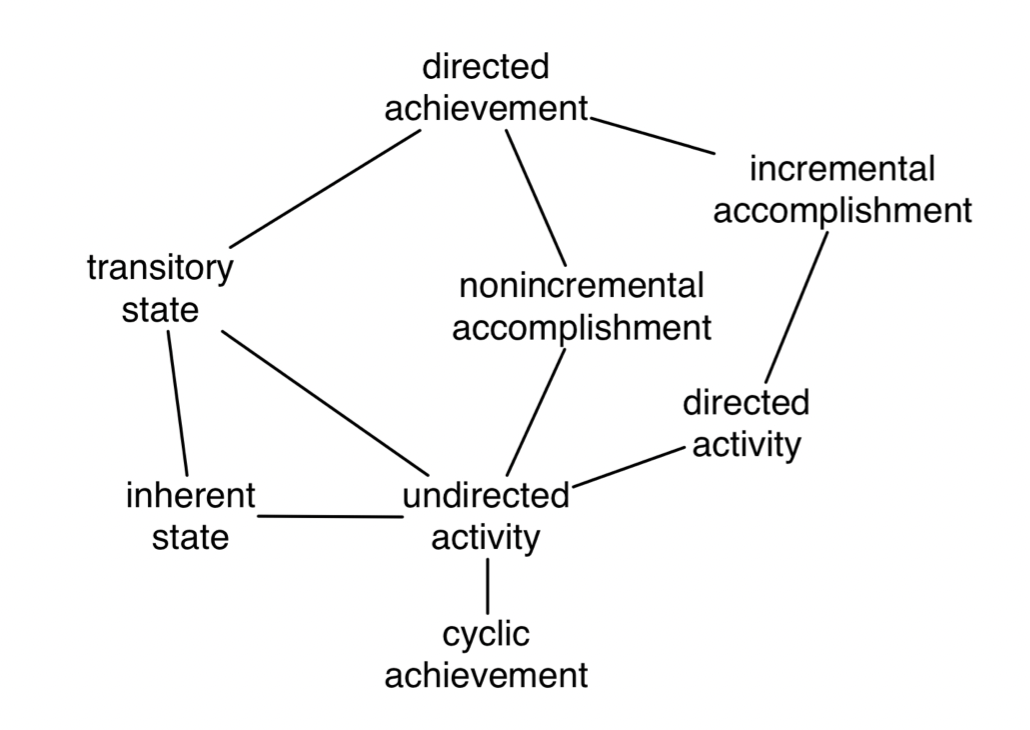
\includegraphics[width=0.5\textwidth]{img/semantic_map.png}
        \centering
        \caption[Semantic map of common aspectual ambiguities]{Croft et al.'s semantic map of common aspectual ambiguities \citet{croft-etal-2016-annotation}}
        \label{fig:semantic_map}
    \end{figure}

    \item \citet{chen-etal-2021-autoaspect} build a rules-based system (or what they call "annotation tool") to predict UMR aspect class, by converting the aspect annotation guidelines into computable steps. Out of 235 gold events distributed across four gold files, the model missed 56 events, successfully identifying 179, and among these 179 identified events, the model accurately labeled 112, resulting in an accuracy rate of 62.57\%. This is the only work so far to my knowledge using the same aspect classification schema as this study, UMR (see \ref{sect:umr}).
    \item One other particularly interesting example is \citet{friedrich-gateva-2017-classification}, who use an English-Czech parallel corpus to leverage the fact mentioned in \ref{sec:asp_in_slav_lang} that Slavic languages such as Czech have two forms of each verb, each assigned to a different aspectual reading depending on the context. This makes it possible to extract aspectual information from a Czech translation of an English sentence, assuming an accurate translation, to use as further training data for their linear regression model. They find that incorporating this "silver-standard" data into their training leads to significant increase in the $F_1$ score, especially when predicting \textsc{atelic} examples.
    
\end{itemize}

\subsection{(L)LMs and aspect}
There have also been attempts to use more modern NLP techniques such as language models for aspect classification and studies probing their aspectual knowledge.
\begin{itemize}
    \item \citet{metheniti-etal-2022-time} carry out a range of experiments with several transformer models (such as BERT, RoBERTa and XLNet) to try and understand to what extent they encode aspectual knowledge. They fine-tune the models on separate classification tasks for telicity and duration, as well as carrying out a qualitative analysis, and come to the conclusion that transformer models \emph{do} understand aspectual phenomena to a sufficient extent, and they find that this knowledge relatively spread across the layers. However, they do not further probe how this information is encoded or which features the model uses to make its decision.
    \item Conversely, however, \citet{katinskaia2024probing} find that in Russian BERT models \citep{kuratov2019adaptation} aspect information is stored in layers higher up. \citet{katinskaia2024probing} also find that their model has high uncertainty when predicting aspect in "alternative contexts" (i.e. where both the imperfective and the perfective verb is possible, depending on the implicit context). On the one hand, this is an encouraging find, as it suggests a correlation between machine behaviour and human behaviour, but on the other hand it is not particularly surprising, since "alternative contexts" are by definition contexts with no tokens containing aspectual information, which are usually used by the model to make a decision. 
    \item \citet{rezaee2021discriminative} look at using generative and discriminative transformers for situation entity classification, which is, however, a slightly different task (see \ref{sect:sit_ent}).
\end{itemize}

\citet{friedrich-etal-2023-kind} notes however that there have still been very little (if any) work looking at the probing or explainability of LMs for this task.

\section{Available datasets}
Although not small in number or size, the available datasets are relatively sparse since there is a very wide range of aspectual phenomena (/schemata) which can be annotated for. For example while some are annotated for aspectual phenomena such as habituality \citep{mathew2009supervised, ikuta-etal-2014-challenges} and others purely for telicity \citep{friedrich-gateva-2017-classification, kober-etal-2020-aspectuality, metheniti-etal-2022-time}, some (generally smaller) datasets are also annotated for a more general schema such as Vendler's classification \citep{zarcone-lenci-2008-computational, hermes_2015, zellers-choi-2017-zero} or Universal Dependencies (UD) aspect classes \citep{kondratyuk-straka-2019-75}. So while there is a relatively wide range of datasets, they are all annotated for slightly different tasks and with different guidelines, which makes matters a little more challenging.

% For reasons explained in \ref{sect:umr}, I decided, like \citet{chen-etal-2021-autoaspect}, to use the UMR aspect lattice as my aspect classification schema, for which however, there only exists one dataset currently \citep{umr}.

For aspect ambiguity the only currently existing annotated dataset of which I am aware is \citet{Friedrich2014AutomaticPO}, which is however only annotated for ambiguity between \textsc{dynamic} and \textsc{stative}. I therefore had to create my own (see \ref{sect:manual_amb_annotation}).

% \section{Formal representations of aspect}
% In this section I will briefly mention some of the attempts to formalise aspect
\section{Related areas of work}
\subsection*{Situation entities}
\label{sect:sit_ent}
Situation entity classification is the task of identifying different types of situations, which exist at a clausal level. The task comes more from the tradition of discourse analysis since it is important for discourse representation theory (DRT) to know, for example, which new referents are introduced to a discourse, and also to analyse temporal relationships. Works usually use the original 8 types introduced by \citet{Smith_2003}: events, states, generalizing sentences, generic sentences, facts, propositions, questions and imperatives. While incorporating concepts from linguistic aspect, the focus is more on a discourse level and the classification schemata are thus different accordingly. Some works in this area include \citet{palmer-etal-2007-sequencing}, \citet{friedrich-etal-2016-situation}, \citet{becker-etal-2017-classifying}, \citet{friedrich2017states} and \citet{dai-huang-2018-building}.

\subsection*{Applications: Temporal reasoning}
An application of the tasks looked at in this chapter and a related area of work is the more general area of temporal reasoning. While this is evidently closer to the area of situation entities introduced in \ref{sect:sit_ent}, the more linguistically-informed side of aspect also has a role to play. For example, it is clear that the two following sentence, differing only in their aspect, refer to two very different events.

\begin{exe}
    \ex The driver of this vehicle drinks wine.
    \ex The driver of this vehicle is drinking wine.
\end{exe}

\citet{costa-branco-2012-aspectual} analyse the importance of aspect for temporal relation classification, and \citet{Derczynski2015TemporalRC} employ a tense and aspect framework to sequence events in text. \citet{Allen2012InterpretingTT} explores various aspects of tense and aspect in event processing. Similarly, \citet{Kamp1993} discusses the integration of tense and aspect information within discourse representation theory (DRT). Furthermore, \citet{kober-etal-2019-temporal} develop a dataset to evaluate the temporal and aspectual entailment capabilities of models. 

More broadly, it is clear that understanding verbal aspect is crucial for a variety of more general downstream tasks, including machine translation and question answering systems. See \citet{friedrich-etal-2023-kind} for a more in-depth look at the applications of this area.